\documentclass[10pt,letterpaper]{article}

\usepackage{hyperref}
\usepackage{cogsci}
\usepackage{pslatex}
\usepackage{pdfsync}
\usepackage{apacite}
\usepackage{amsmath}
\usepackage{graphicx}
\usepackage{topcapt}
\usepackage{color}


\title{(title-in-progress:) Felicity ratings of negative sentences in context}
 
\author{{\large \bf Ann E. Nordmeyer} \\ \texttt{anordmey@stanford.edu}\\ Department of Psychology \\ Stanford University \\ 
\And {\large \bf Michael C. Frank} \\ \texttt{mcfrank@stanford.edu} \\ Department of Psychology \\ Stanford University \\ }

\begin{document}

\maketitle


\begin{abstract}
Why are negative sentences processed faster in some contexts than in others?  Previous work suggests that the effects of context on negative sentence processing are due to the informativeness of negation in context \cite{nordmeyer2014}.  We explored how adults' explicit felicity judgments changed depending on the context in which a negative sentence was presented.  In Study 1, we found that negative sentences were rated as more felicitous when they were presented within a strong context compared to a weak context, and that negative sentences expressing nonexistence were rated higher than negative sentences that referred to an alternative object.  In Study 2, we found that negative sentences referring to an alternative characteristic were rated higher when they were presented in a context where all of the other characters possessed the negated object, compared to contexts where the other characters possessed the alternative object or no object.  Finally, we compared these data to a model of the informativeness of sentences in context, and found that this model reflected the same pattern as adults' ratings for true negative sentences in our experiments.  Our data suggest that the felicity of negative sentences may be influenced by their informativeness in context.  


\textbf{Keywords:} 
Negation; felicity judgments; pragmatics
\end{abstract}

\section{Introduction}

An important aspect of human communication is how speakers use language and how listeners interpret their intended meaning.  A sentence that is perfectly grammatical can sound strange depending on the context.  If you open a mysterious box and find that it is empty, it would be odd for to say ``This box doesn't contain any chocolates''.  If you are in a chocolate store, however, and are surrounded by boxes filled with chocolate, this same sentence suddenly becomes a perfectly reasonable thing to say.  Why do some sentences sound strange in one situation, but normal in another?

Negation makes a good case study to examine the effects of context on sentence judgments because, as the previous example demonstrates, negative sentences are particularly sensitive to to effects of context.  Previous work on sentence processing suggests that negative sentences take much longer to evaluate compared to positive sentences when they are presented without any context \cite{hclark1972, carpenter1975, just1971, just1976}.  When participants are presented with supportive contextual information -- specifically, context that sets up an expectation that is violated -- the time to process a negative sentence is significantly reduced \cite{wason1965, glenberg1999, ludtke2006, nieuwland2008, dale2011, nordmeyer2014b}.  

The context of a negative sentence can also influence the type of negation that the sentence expresses.  Most of the previous work on adults' comprehension of negative sentences has focused on denial, or truth-functional negation -- that is, negative sentences expressing that some proposition is false \cite<cf.>{nordmeyer2014}.  This is not the only function of negation, however; negative sentences can be used to express nonexistence, refusal, and prohibition, among many others \cite<see>{choi1988}.  Here, we focus \emph{negation-as-alternative} and \emph{negation-as-nonexistence} ((NOTE: I am getting a little bogged down by terminology in this paper -- starting here, but especially when I start describing different conditions later.   Any suggestions??)), which can be expressed with the same sentence depending on the context.  Referring to our previous example, the sentence ``This box doesn't contain chocolate'' might referring to the fact that the box is empty (conveying nonexistence), but it could be referring to the fact that the box contains some alternative object (e.g. the box contains broccoli, not chocolate!).  

Much of the literature on how people use different types of negation has focused on children's production of negation \cite{bloom1970, pea1980, choi1988}.  In one study, children in an eye-tracking study heard sentences such as ``Look at the boy who has no apples'', where the target of the sentence was either a character with nothing (negation-as-nonexistence) or a character with some other object (negation-as-alternative) \cite{nordmeyer2013, nordmeyer2014b}.  Children had more difficulty identifying the referent of the negative sentence when the negation referred to nonexistence, possibly due to the task demands involved in orienting away from a more engaging picture.  Adults, however, were marginally faster to orient towards the correct picture in the negation-as-nonexistence condition compared to the negation-as-alternative condition.  This suggests that adults are sensitive to this difference, but it is not clear if this is due to differences in processing demands (e.g. adults may have found it easier than children to identify a character with nothing, compared to a character with a different object), or if this reflects an expectation that adults have about how negation should be used in different contexts.  Adults' may have found the negative sentences infelicitous in the negation-as-alternative context, because they expected the sentence to describe the feature that the character \emph{had}, rather than a feature that they did \emph{not} have.

Why might different contexts influence the processing of negation?  According to Grice's Cooperative Principle \cite{grice1975}, speakers should produce utterances that are truthful, relevant, and informative.  In previous work, we demonstrated that negative sentences are more informative in contexts that set up a strong expectation that is violated, and that this difference in informativeness can predict adults' reaction times to respond to negative vs. positive sentences \cite{nordmeyer2014}.  In this paper, we explore the effects of context on adults' explicit felicity judgments for different types of negative sentences.  In Study 1, we test the effect of a strong vs. a weak context on two different types of negative sentences: negation-as-nonexistence and negation-as-alternative.  We also tested two different negative sentence frames: ``has no'' and ``doesn't have''.  We found that negative sentences presented in a strong context were rated higher than negative sentences in a weak context, and that negation-as-nonexistence sentences were rated higher than negation-as-alternative sentences.  In Study 2, we focused on negation-as-alternative trials to further explore how context influences the felicity of these sentences.  We found that these sentences are rated higher when they were presented in a context where all of the other characters possessed the negated object, compared to contexts where the other characters possessed the alternative object or no object.  Finally, we found that a model of the informativeness of sentences in context predicted the same qualitative pattern seen in our data, suggesting that adults' felicity judgments reflect preferences for sentences that are more informative given the context.


Why we did this study.
\section{Study 1}

Study 1 explored how different contexts affected participants felicity ratings for negative sentences.  Half of the participants in Study 1 saw sentences presented within a weak context (e.g. one where none of the context characters had any objects), and the other half saw sentences presented within a strong context (e.g. one where everyone in the context possessed the negated object).  Previous work has found that this context manipulation improves adults' processing of negative sentences \cite{nordmeyer2014}; here we test whether context changes explicit felicity judgments as well.  

We also tested two within-subjects factors that might influence negative sentence ratings.  First, we looked at how different syntactic framings might influence sentence judgments.  In our previous work on the effects of context on reaction time, we tested sentences such as ``X has no Y''.  In this experiment, we also tested sentential negation, using sentences such as ``X doesn't have Y''.  We were interested in whether participants had a preference for one framing over another, and whether this would interact with context.  If previously seen context effects are driven by the informativeness of negation in different contexts, then these same effects should appear regardless of the syntactic framing of the sentences.  

Finally, we examined whether the type of negation influenced felicity.  In half of the true negative trials, the referent of the negative sentence was a character who had nothing.  In these sentences, the negation refers to the \emph{nonexistence} of the named item.  In the other half of true negative trials, the referent of the sentence was a character who had some other object.  In these sentences, the negation refers to the fact that the character has an \emph{alternative} object.  Previous work suggests that children and adults show different gaze patterns in response to these different types of negative sentences \cite{nordmeyer2014b}; here we explore whether adults' have a preference for the type of negation expressed in different negative sentences.

\subsection{Method}

\subsubsection{Participants}
We recruited 94 participants to participate in an online experiment through the Amazon's Mechanical Turk (mTurk) website.  Participants ranged in age from 18-65; 50 male and 41 female (3 declined to report gender).  We restricted participation to individuals in the United States. We paid participants 35 cents to participate, which took approximately 5 minutes to complete.  


\subsubsection{Stimuli}
We created sixteen trial items.  On each trial, four different Sesame Street characters were shown standing behind tables.  One character was randomly selected as the "target" character, designated by a red box around that character \& the character's table, and the remaining three characters were designated as "context" characters.

Participants were randomly assigned to the ``no context'' condition or the ``context'' condition.  In the no context condition, the context characters all stood behind empty tables.  In the context condition, each context character had identical objects on their tables (``target objects'').  The objects belonged to one of four categories: animals (cat, dog, horse cow), vehicles (car, bus, boat, truck), food (apple, banana, cookie, orange), and household objects (fork, spoon, bowl, plate).  

Below the characters was a sentence about the target character.  Six of these sentences were positive sentences of the form ``[CHARACTER] has a/an [TARGET OBJECT].''  Five were negative sentences of the form ``[CHARACTER] has no [TARGET OBJECT]'' and five were negative sentences of the form ``[CHARACTER] doesn't have a/an [TARGET OBJECT]''.  

The target character either had a target object on their table, or an alternative object (``alternative'' trials), or nothing (``nonexistence'' trials).  This allowed us to examine two different negative concepts (negation-as-alternative and negation-as-nonexistence).  These trial conditions were crossed such that each participant saw six true positive trials, two false positive trials (one ``alternative'' and one ``nonexistence''), two false negative trials (one ``has no'' sentence type and one ``doesn't have'' sentence type), and eight true negative trials (two ``has no''/nonexistence, two ``has no''/alternative, two ``doesn't have/nonexistence'', and two ``doesn't have/alternative'').  Each of these trial types was randomly assigned to a target object, and trials were presented in a random order.

A slider bar was positioned beneath the sentence, with a 7 point scale ranging from ``Very Bad'' to ``Very Good''.  A progress bar at the top of the screen informed participants how much of the experiment they had completed. 

\begin{figure}[t]
\begin{center} 
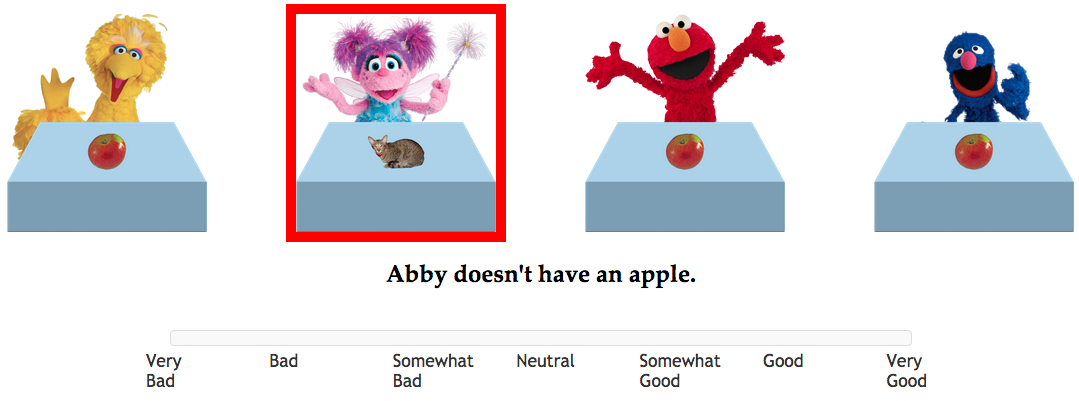
\includegraphics[width=3.25in]{figures/example.png}
\caption{\label{fig:trial} A "true negative" trial with the alternative negation type.}
\vspace{-5mm}
\end{center} 
\end{figure}

\subsubsection{Procedure}
Participants were first presented with an instructions screen that briefly described the task and informed them that they could stop at any time.  Once participants had agreed to participate in the task, they saw an instructions screen that explained the task in more detail.  The instructions explained that participants would see a sentence, and that this sentence was about the character in the red square.  Participants were told that their job was to rate how ``good'' each sentence is, and ``if no one would ever say a particular sentence in this context, or if it is just wrong, rank that as `Very Bad', but if something is right and sounds perfectly normal, mark it as `Very Good'.''  Participants were encouraged to use the entire scale to make their ratings.

On each trial the pictures, sentence, and slider bar appeared simultaneously, and participants had to make a selection on the sliding scale in order to progress to the next trial.  

\subsubsection{Data Processing}
We excluded from analysis two participants who did not list English as their native language, and eight participants for using fewer than 3 points on the scale.  Thus, data from a total of 84 participants were analyzed, 46 in the no context condition and 38 in the context condition.  

\subsection{Results \& Discussion}

\subsubsection{All sentences}

True negative sentences were rated significantly higher when they were presented in a strong context compared to a weak context (see Figure \ref{fig:s1}), supporting our hypotheses and previous research on the effects of context on negation.  True positive sentences did not show any effect of context, nor did false sentences of any sentence type, likely due to a ceiling effect for true positive sentences and a floor effect for false sentences.  

We ran a linear mixed-effects model testing the interaction between context, sentence type, and truth value on participant sentence ratings.\footnote{All mixed-effects models were fit using the lme4 package in R version 2.15.3.  The model specification was as follows: \texttt{rating $\sim$ context~$\times$~sentence~$\times$~truth + (sentence~$\times$~truth~\textbar~subject) +  (sentence~$\times$~truth~\textbar~item)}  Significance was calculated using the standard normal approximation to the $t$ distribution \cite{barr2013}. Data and analysis code can be found at \href{http://github.com/anordmey/FILLTHISIN}{http://github.com/anordmey/FILLTHISIN}}.  Results of this model showed a main effect of sentence type, with negative sentences receiving significantly lower ratings than positive sentences ($\beta= -.58$, $p< .01$), and a main effect of truth value, with false sentences scoring approximately four points lower on the 7-point scale compared to true sentences ($\beta= 4.19$, $p< .001$).  There was not a main effect of context ($\beta= -0.52$, $p=.12$), but there was a significant interaction between sentence type and context, with negative sentences scoring significantly higher when presented in a strong context compared to a weak context ($\beta= 2.04$, $p< .05$).  

These results confirm that the effects of context seen in the sentence processing literature are also manifested in participants' explicit felicity ratings.  Participants rated true negative sentences as better when the other characters in the context had the negated item.  For example, the sentence ``Abby has no apples'' was rated higher when all of the other characters \emph{had} apples, compared to contexts where all of the other characters had nothing.  (MORE HERE)

\subsubsection{True negative sentences}

Negative sentences expressing nonexistence were rated as more felicitous than negative sentences that referred to an alternative object, and sentences with the framing ``doesn't have'' were rated higher than sentences with the framing ``has no''.  These effects persisted regardless of whether the sentence was presented in a weak context or a strong context (see Figure \ref{fig:s1}).  

To test the reliability of these findings, we fit a linear mixed-effects model to sentence ratings for responses to true negative sentences only.  Coefficients for this model can be seen in Table \ref{tab:s1}.  We examined the interaction between context, negation type (e.g. nonexistence or alternative), and negation framing (e.g. ``has no X'' vs ``doesn't have X'').\footnote{ The model specification was as follows: \texttt{rating $\sim$ context~$\times$~negation type~$\times$~negation type + (negation type~$\times$~negation frame~\textbar~subject) +  (negation type~$\times$~negation frame~\textbar~item)}} We found a main effect of context, with true negative sentences presented in a strong context eliciting significantly higher ratings than true negative sentences presented in a weak context ($\beta= .99$, $p< .001$).  We also found main effects of negation type, with sentences referring to an alternative receiving lower ratings than sentences expressing nonexistence ($\beta= -.46$, $p< .05$), as well as negation framing, with sentences of the form ``has no X'' receiving lower ratings than sentences of the form ``doesn't have X''  ($\beta= -.46$, $p< .05$).  There were no interactions between negation frame, negation type, and context.  

The difference between the two negation sentence frames is likely due to frequency effects in the input (GET SOME DATA). 

The fact that negative sentences expressing nonexistence were rated higher than negative sentences referring to an alternative property reflects previous findings from eye-tracking experiments testing the same difference \cite{nordmeyer2014b}.  In that study, adults were marginally faster to look at the target of a negative sentence when that sentence referred to nonexistence compared to when the sentence referred to an alternative property.  These data suggest that this finding is not merely due to superficial differences in between the stimuli (e.g. it is easier to identify a character with nothing than a character with a different object), but perhaps because the nonexistence condition was more felicitous than the alternative condition.  (((NOTE: Is this too much of a stretch?))) 

One explanation for this finding is that a negative sentence such as ``Abby doesn't have an apple'' is more informative when Abby has nothing compared to when she has an alternative object.  In a strong context (e.g. one where everyone besides Abby has apples), using negation to point out Abby's lack of apples is informative, because it uniquely identifies her character in the array.  When Abby has some alternative object (e.g. a cat), however, there is a \emph{more} informative utterance that a speaker could use (e.g. ``Abby has a cat'').  The presence of a more informative utterance makes these negative sentences less felicitous, even when they appear in a strong context.


((TRANSITION TO STUDY 2))


\begin{figure}
\begin{center} 
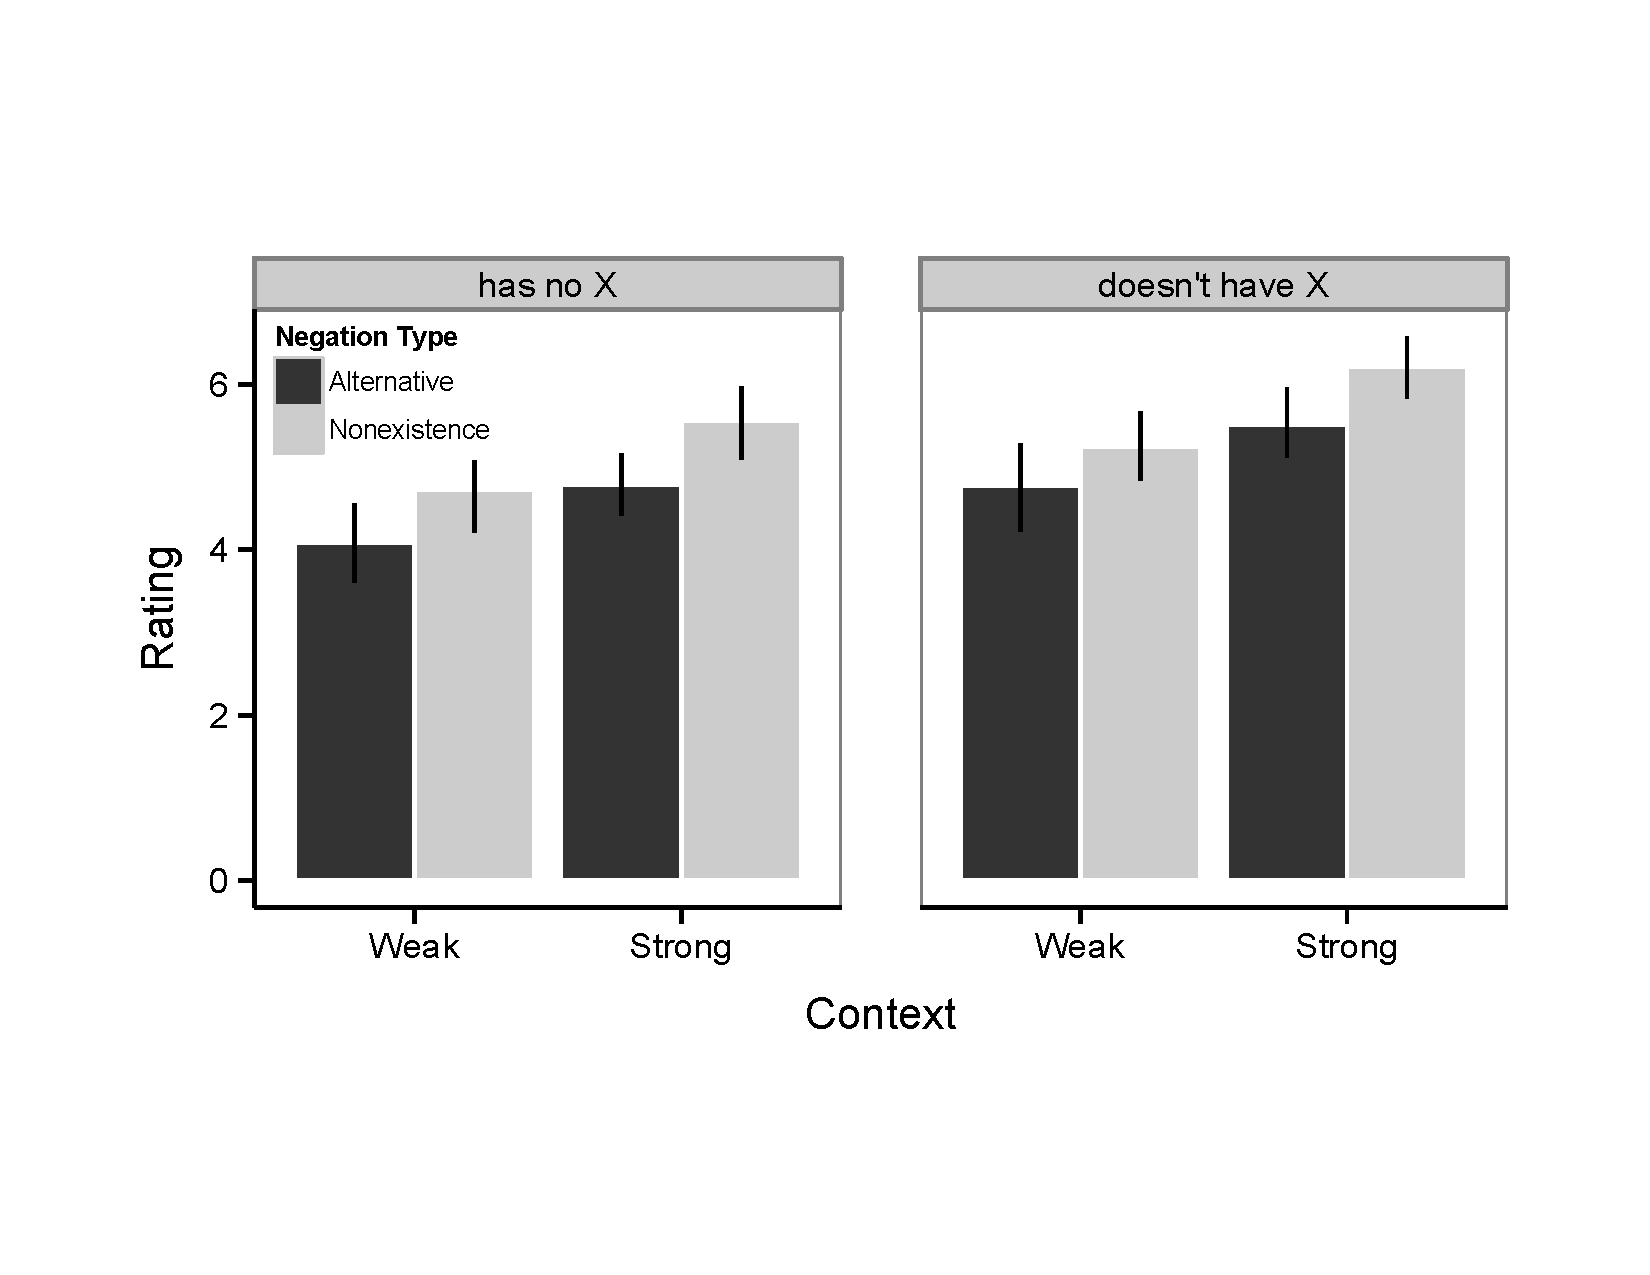
\includegraphics[width=3.25in]{figures/study1.pdf}
\caption{\label{fig:s1} Ratings for different types of true negative sentences in Study 1.  Sentences of the form ``...has no X'' are shown on the left, and sentences of the form ``doesn't have X'' are shown on the right.  Negative sentences expressing nonexistence are shown in black, and negative sentences referring to an alternative object are shown in gray.  Error bars show 95\% confidence intervals.}
\end{center} 
\end{figure}

\begin{table}[t]
\caption{\label{tab:s1} Coefficient estimates from a mixed-effects model predicting ratings for true negative sentences in Study 1.}
\begin{center}
\small\addtolength{\tabcolsep}{-5pt}
\begin{tabular}{rrrr}
  \hline
 & Coefficient & Std. err. & t value \\ 
  \hline
(Intercept) & 5.24 & 0.20 & 25.94 \\ 
  Context (strong) & 0.99 & 0.29 & 3.46  \\ 
  Negation type (alternative) & -0.46 & 0.18 & -2.51 \\
  Frame (``has no'') & -0.51 & 0.25 & -2.01 \\ 
  Context $\times$Negation type & -0.32 & 0.24 & -1.32 \\
  Context $\times$Frame & -0.18 & 0.35 & -0.50 \\
  Negation type$\times$Frame & -0.19 & 0.22 & -0.83 \\
  Context$\times$Negation type$\times$Frame & 0.20 & 0.33 & 0.62 \\
   \hline
\end{tabular}
\vspace{-1.5cm}
\end{center}
\end{table}

\section{Study 2:}

Study 1 found clear differences in participants' ratings of negative sentences.  Participants preferred negative sentences with the sentential framing ``doesn't have X'' compared to the lexical framing ``has no X''.  Participants also preferred negative sentences that referred to nonexistence.  Across both of these factors, negative sentences that were presented within a strong context (where all context characters possessed the negated object) received higher ratings than negative sentences presented in a weak context, where none of the characters in the context possessed any object.

In the next study, we further explore this context effect by focusing specifically on negation-as-alternative sentences with a ``doesn't have'' framing.  In Study 2, we made context a within-subjects factor, so that participants saw multiple items of different context types throughout the experiment.  We examined the effect of three different types of context: a ``target'' context, in which all context characters had the negated target object (identical to the strong context in Study 1), a ``none'' context, in which none of the context characters had any objects (identical to the weak context in Study 1), and a ``foil'' context, in which all context characters had an alternative object (e.g. a different object than the one negated in the negative sentences). 

We expected to replicate the same difference between the none context and the target context as was seen in Study 1: Negative sentences presented in a target context should receive higher ratings than negative sentences presented in a none context.  We had two competing predictions about the foil context ((NOTE: I actually didn't articulate this until after running the experiments, but I think it works as a possible alternative hypothesis.  Is it OK to set this up like this))).  In true negative trials with a foil context, all characters (including the target character) had the same objects on their table (e.g. cats), and the negative sentence referred to a different object (e.g. ``X doesn't have apples'').  Some previous work has suggested that a critical element of the effect of context on negative sentences is the fact that the referent of the negative sentence is the ``odd one out'' \cite{wason1965}.  If this is the case, the foil context might be even worse than the none context, because the target of the negative sentence does not stand out from the context.  If, however, the mechanism by which context influences negation is the fact that context changes the informativeness of negation, then there should be no difference between the foil and none contexts, because negative sentences are no less informative in the foil context.  

\subsection{Method}

\subsubsection{Participants}
We recruited 194 participants to participate in an online experiment through the Amazon's Mechanical Turk (mTurk) website.  Participants ranged in age from 18-65; 115 male and 76 female (3 declined to report gender).  We restricted participation to individuals in the United States. We paid participants 40 cents to participate, which took approximately 7 minutes to complete.  


\subsubsection{Stimuli}
Trials in Study 2 had the same structure as trials in Study 1, with the following exceptions:

We created 24 trials for Study 2.  All negative sentences were of the form ``[CHARACTER] doesn't have a/an [TARGET OBJECT]''.  On each trial, the target character either had a target item on their table, or had an alternative item (eliminating the negation-as-nonexistence trials).  Each participant evaluated nine true positive sentences, three false positive, three false negative, and nine true negative trials.

In Study 2, context was a within-subjects factor with three levels.  Trials either had no context (e.g. context characters had nothing on their table, identical to the no context condition in Study 1), target context (i.e. context characters each had a target item on their table, same as the context condition in Study 1), or a foil context (i.e. context characters had an alternative item on their table, e.g. all characters have cats, and the sentence is about the presence/absence of apples).  Each context condition appeared an equal number of times within each trial type.  

\subsubsection{Procedure}
The procedure was identical to Study 1.

\subsubsection{Data Processing}
We excluded from analysis four participants who did not list English as their native language, six participants for having participated in a previous pilot study, and 34 participants for using fewer than 3 points on the scale.  Thus, data from a total of 154 participants were analyzed.  

\subsection{Results \& Discussion}
True negative sentences were rated significantly higher when they were presented in a strong target context compared to either the none context or the foil context (see Figure \ref{fig:modelvdata}).  Negative sentences presented in a foil context received a very small increase in ratings compared to negative sentences presented in a none context ((NOTE: I'm in a weird position here where it REALLY does not look like there is a significant difference here (I actually initially wrote that there WASN'T a difference), but it does show up as marginally significant in my data (and actually significant if I run a model on just the true sentences, which I don't report here but did on my own).  So I feel weird describing this as an actual difference in this first paragraph, but it does show up in my data -- and also in my model -- so I feel like I should?))).  As in Study 1, there was no effect of context on true positive sentences or false sentences.  

We fit a linear mixed-effects model to sentence ratings to test the interaction between context, sentence type, and truth value.\footnote{ The model specification was as follows: \texttt{rating $\sim$ context~$\times$~sentence type~$\times$~truth value + (sentence type~$\times$~truth value~\textbar~subject) +  (sentence type~$\times$~truth value~\textbar~item)}}  Coefficients for this model can be seen in Table \ref{tab:s2}.  We found a significant effect of truth value, with true sentences receiving significantly higher ratings than false sentences, ($\beta= 5.01$, $p< .001$).  A significant interaction between sentence type and truth value indicates that true negative sentences received lower ratings than true positive sentences, ($\beta= -1.78$, $p< .001$).  Finally, a three-way interaction between between sentence type, truth value, and context was significant for the target context ($\beta= 1.08$, $p< .001$), and marginally significant for the foil context ($\beta= .34$, $p=.06$), indicating that true negative sentences received significantly higher ratings in the target context compared to the none context, and slightly higher ratings in the foil context compared to the none context.  


\begin{table}[t]
\caption{\label{tab:s2} Coefficient estimates from a mixed-effects model predicting sentence ratings in Study 2.}
\begin{center}
\small\addtolength{\tabcolsep}{-5pt}
\begin{tabular}{rrrr}
  \hline
 & Coefficient & Std. err. & t value \\ 
  \hline
(Intercept) & 1.62 & 0.11 & 15.07 \\ 
  Context (foil) & 0.13 & 0.11 & 1.14  \\ 
  Context (target) & 0.05 & 0.11 & 0.43  \\ 
  Sentence type (negative) & 0.11 & 0.12 & 0.94 \\
  Truth value (true) & 5.01 & 0.13 & 37.60 \\ 
  Context (foil)$\times$Sentence & -0.16 & 0.16 & -0.98 \\
  Context (target)$\times$Sentence & -0.11 & 0.16 & -0.72 \\
  Context (foil)$\times$Truth & -0.19 & 0.13 & -1.48 \\
  Context (target)$\times$Truth & -0.14 & 0.13 & -1.08 \\
  Sentence$\times$Truth & -1.78 & 0.16 & -11.40 \\
  Context (foil)$\times$Sentence$\times$Truth& 0.34 & 0.18 & 1.87 \\
  Context (target)$\times$Sentence$\times$Truth & 1.08 & 0.18 & 5.88 \\
   \hline
\end{tabular}
\vspace{-1.5cm}
\end{center}
\end{table}

DISCUSSION HERE


\section{Model}

Studies 1 and 2 explored the effects of context on different types of negative sentences.  Both studies found a significant effect of context on participants' ratings of true negative sentences.  Why does context have this effect on negative sentences?  One possibility is that felicity ratings are influenced by the \emph{informativeness} of negative sentences.  According to \citeNP{grice1975}, speakers should produce sentences that are appropriately informative based on the context.  In a context where most characters have apples and another character has a cat, it is informative to mention the ``odd character out'' by describing the cat, because this feature is unique to the character being described.

Previous work suggests that listeners expect speakers to produce informative utterances \cite{frank2012}, and that this can predict adults' speed to evaluate negative sentences \cite{nordmeyer2013}.  Here, we use the same model to explore whether participants' felicity judgments can be predicted by the informativeness of those sentences in context.  We focus on true negative sentences here, because the ceiling effect for true positive sentences and the floor effect for negative sentences make it difficult to consider the effect of context on these sentences.  

((NOTE: CHANGE THIS: Describe more generally))
We modeled the behavior of participants in our experiments by assuming that participants' felicity judgments are proportional to the probability of the utterance $w$, given the context $C$ and the speaker's intended referent $r_S$:

\noindent We then define the probability of the utterance as proportional to its utility (following \citeNP{frank2012}):

\begin{equation}\label{eq:pw1}
P(w | r_s, C) \propto  e^{U(w;r_s,C)},
\end{equation} 

\noindent This utility is defined as the informativeness of $w$ minus its cost $D(w)$:

\begin{equation}\label{eq:utility}
U(w;r_s,C) = I(w;r_s, C) - D(w).
\end{equation}

\noindent Informativeness in context is calculated as the number of bits of information conveyed by the word. We assume that $w$ has a uniform probability distribution over its extension in context (e.g.\ ``has apples'' applies to any character who has apples, leading to a probability of $1/|w|$ of picking out each individual character with apples) :

\begin{equation}\label{eq:info}
I(w;r_s, C) = -(-\log(|w|^{-1})).
\end{equation}

We created a sparse vocabulary which represented possible words to describe the characters.  This included the target utterance (e.g.\ ``has apples'' and ``doesn't have apples''), an utterance referring to the alternative item (e.g. ``has cats''/``doesn't have cats''), as well as words that were uniformly true or false of all characters. Normalizing Eq.\ \ref{eq:pw1} over all possible words in the vocabulary $V$, we have:

\begin{equation}\label{eq:pw2}
P(w | r_s, C) = \frac{ e^{\log(|w|^{-1}) - D(w)}} {\sum_{w' \in V}{e^{\log(|w'|^{-1}) - D(w')}}}.
\end{equation}

\begin{figure}
\begin{center} 
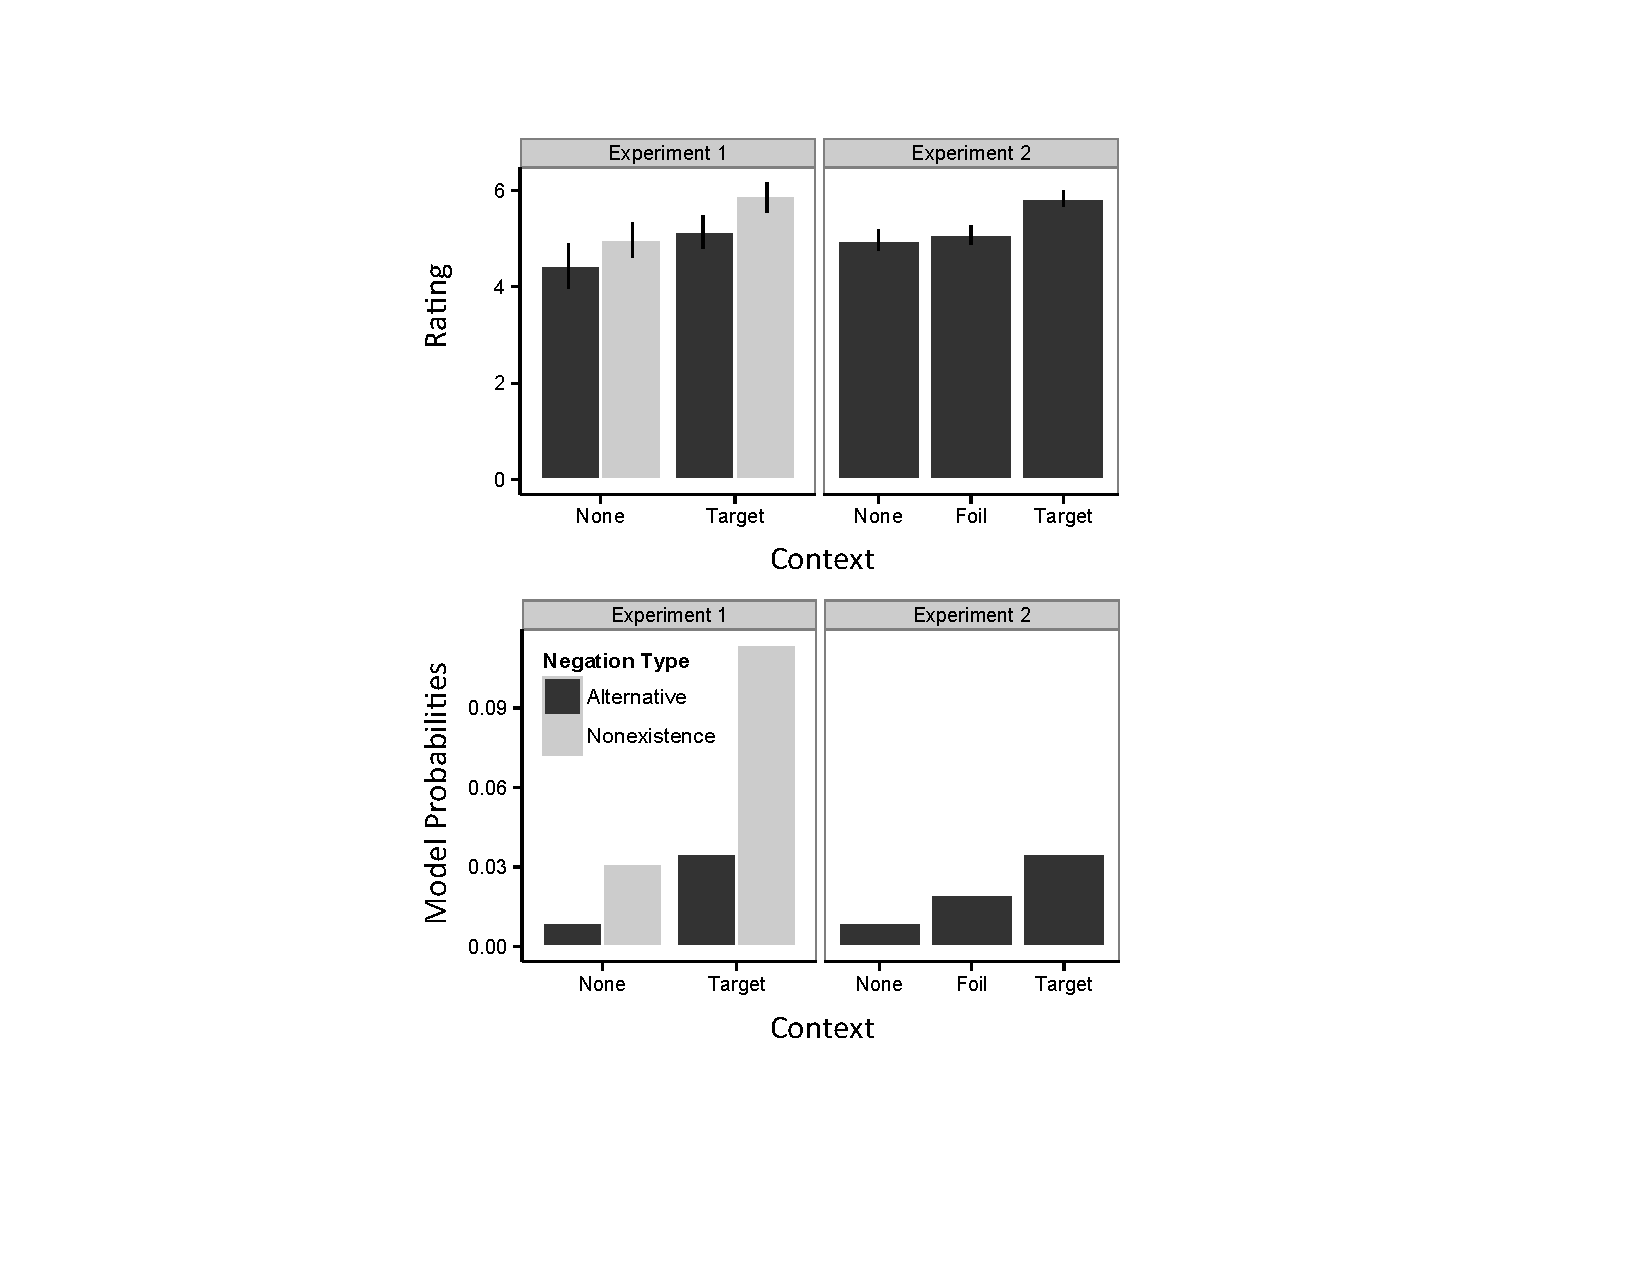
\includegraphics[width=3.25in]{figures/modelcomp.pdf}
\caption{\label{fig:modelvdata} CAPTION HERE.}
\end{center} 
\end{figure}

DISCUSS THINGS HERE.

\section{General Discussion}

\bibliographystyle{apacite}

\setlength{\bibleftmargin}{.125in}
\setlength{\bibindent}{-\bibleftmargin}

\bibliography{bibLibrary}


\end{document}
